\chapter{Hopping sites}
\label{sec:mapping}

\section{Conjugated segments and rigid fragments}
\label{sec:conjugated_segments}

\begin{wrapfigure}{ht}{0.5\linewidth}
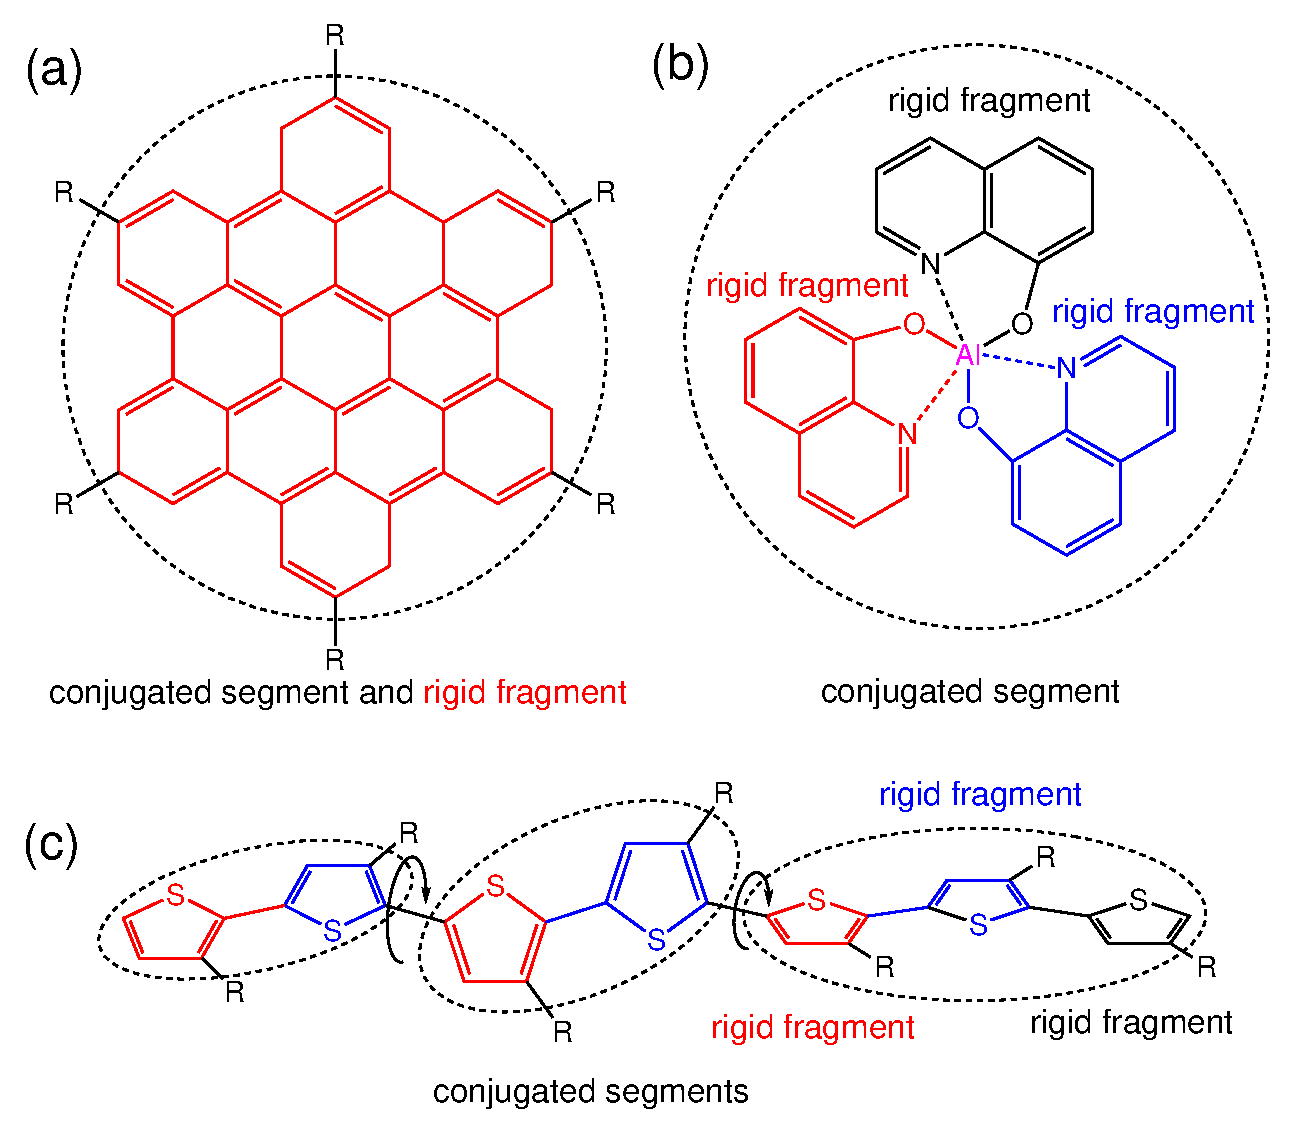
\includegraphics[width=\linewidth]{fig/conjugated_segment/fragment_segment}
\caption{\small The concept of conjugated segments and rigid fragments. Dashed lines indicate conjugated segments while colors denote rigid fragments. (a) Hexabenzocoronene: the $\pi$-conjugated system is both a rigid fragment and a conjugated segment. (b) \Alq: the Al atom and each ligand are rigid fragments while the whole molecule is a conjugated segment. (c) Polythiophene: each repeat unit is a rigid fragment. A conjugated segment consists of one or more rigid fragments. One molecule can have several conjugated segments.}
\label{fig:segment}
\end{wrapfigure}

With the morphology at hand, the next step is partitioning the system on hopping sites, or conjugated segments, and calculating charge transfer rates between them. Physically intuitive arguments can be used for the partitioning,  which reflects the localization of the wave function of a charge. For most organic semiconductors, the molecular architecture includes relatively rigid, planar $\pi$-conjugated systems, which we will refer to as rigid fragments. A conjugated segment can contain one or more of such rigid fragments, which are linked by bonded degrees of freedom. The dynamics of these degrees of freedom evolves on timescales much slower than the frequency of the internal promoting mode. In some cases, e.g. glasses, it can be `frozen' due to non-bonded interactions with the surrounding molecules.

To illustrate the concept of conjugated segments and rigid fragments, three representative molecular architectures are shown in \fig{segment}. The first one is a typical discotic liquid crystal, hexabenzocoronene. It consists of a conjugated core to which side chains are attached to aid self-assembly and solution processing. In this case the orbitals localized on side chains do not participate in charge transport and the conjugated $\pi$-system is both, a rigid fragment and a conjugated segment. 
%
In \Alq, a metal-coordinated compound, a charge carrier is delocalized over all three ligands. Hence, the whole molecule is one conjugated segment. Individual ligands are relatively rigid, while energies of the order of $k_\text{B}T$ are sufficient to reorient them with respect to each other. Thus the Al atom and the three ligands are rigid fragments.
%
In the case of a conjugated polymer, one molecule can consist of several conjugated segments, while each backbone repeat unit is a rigid fragment. Since the conjugation along the backbone can be broken due to large out-of-plane twists between two repeat units, an empirical criterion, based on the dihedral angle, can be used to partition the backbone on conjugated segments~\cite{ruehle_multiscale_2010}. However, such intuitive partitioning is, to some extent, arbitrary and shall be validated by other methods~\cite{vukmirovi_charge_2008,vukmirovi_charge_2009,mcmahon_ad_2009}. 

After partitioning, an additional step is often required to remove bond length fluctuations introduced by molecular dynamics simulations, since they are already integrated out in the derivation of the rate expression. This is achieved by substituting respective molecular fragments with  rigid, planar $\pi$-systems optimized using first-principles methods. Centers of mass and gyration tensors are used to align rigid fragments, though a custom definition of local axes is also possible. Such a procedure also minimizes discrepancies between the force-field and first-principles-based ground state geometries of conjugated segments, which might be important for calculations of electronic couplings, reorganization energies, and intramolecular driving forces. 

Finally, a list of neighboring conjugated segments is constructed. Two segments are added to this list if the distance between centers of mass of {\em any} their rigid fragments is below a certain cutoff. This allows neighbors to be selected on a criterion of minimum distance of approach rather than center of mass distance, which is useful for molecules with anisotropic shapes.

\section{Mapping the system onto conjugated segments}

\texttt{ctp\_map} partitions the system on conjugated segments and rigid fragments
\begin{verbatim}
  ctp_map --top topology.tpr -c 15 -cg cgmap.xml --trj traj.trr
\end{verbatim}
The input are the gromacs topology and trajectory files, a mapping file, a cutoff distance for defining nearest neighbours and a file describing the charge unit types. 

\subsection{The mapping file}
To partition the system onto conjugated segments and rigid fragments a mapping \xml file is required. This file is based on the input provided for generation of \texttt{topol.tpr} and \texttt{traj.trr} files. An example of a mapping file for a single \dcvt molecule is shown in listing~\ref{list:map}.

%\begin{table}
{\small 
\begin{tabular}{p{3cm} p{10cm}}
\xml tag & Description \\
\hline
\texttt{name} & Name of the molecule in the coarse-grained model. Useful for multicomponent systems. \\
%
\texttt{ident} & Name (identification) of the molecule in the all-atom representation. This \emph{must} match the molecule name in the atomistic representation (e.g. \gromacs topology). \\
%
\texttt{topology} & Section describing the partitioning of the molecule on rigid fragments (beads). Atom and residue names/types \emph{must} correspond to those used in the atomistic representation (e.g. \gromacs topology)\\
& \\
\texttt{cg\_beads} & Section describing the different coarse-grained beads (rigid fragments) a molecule or polymer chain may consist of. \\
%
\texttt{cg\_bead} & Section defining one particular bead. \\
%
\texttt{cg\_bead.name} &  The name of the bead. This must be unique for each bead in a molecule. So a polymer made of 10 repeat units needs 10 different bead name identifiers. \\
%
\texttt{cg\_bead.type} &  The type of the bead. This may be the same for beads which only differ by a hydrogen atom or two to simplify the interactions, while the mapping must take such tiny differences into account. \\
%
\texttt{cg\_bead.mapping} & The type of the mapping. Different beads may have the same mapping, since a molecule may contain multiple beads of the same type, but in the bead definition each must correspond to different atoms. \\
%
\texttt{cg\_bead.beads} &  Precise mapping. Lists the molecule labels used in \emph{Gromacs} which form the bead. Note: The first three atoms are used to calculate vectors defining the orientation of the molecule so they must not lie on the same axis. Also the first three atoms in the mapping need not correspond to the first three in the \emph{rtp} or \emph{gro} file, but this mapping must be consistent with the definitions in the list\_charges definition. \\
%
\texttt{cg\_bead.symmetry} &  The symmetry of the molecule. 3 = ellipsoidal with three different axes. \\
& \\
\texttt{qm} & This section associates beads (rigid fragments) with a particular charge unit type \\
%
\texttt{qm.crgunitname} &  The name of the charge unit type the fragment is associated with \\
%
\texttt{qm.bead} & The position of the fragment in the charge unit type. \\
& \\
\texttt{maps} & Section describing the different mapping for all types of beads. \\
%
\texttt{map} &  Section defining one particular map (used to determine the center of a fragment). \\
%
\texttt{map.name} & The name of the mapping. Must correspond to a name used to define the beads above. \\
%
\texttt{map.weights} & The weighting of the atoms inside the bead, usually taken to be the mass of the nucleus in atomic mass units. The weights must be in the same order as the corresponding bead definition.
\end{tabular}
}
%\end{table}

\clearpage

\definecolor{gray}{rgb}{0.4,0.4,0.4}
\definecolor{darkblue}{rgb}{0.0,0.0,0.6}
\definecolor{cyan}{rgb}{0.0,0.6,0.6}

\lstset{
  language=XML,
  frame=lines,
  basicstyle=\ttfamily\footnotesize,
  identifierstyle=\color{red},
  keywordstyle=\color{blue},
  showstringspaces=false,
  columns=fullflexible,
  commentstyle=\color{gray}\rmfamily\itshape,
  morekeywords={cg_molecule,cg_beads,cg_bead,crgunitname,bead,beads,type,topology,name,ident,maps,map,mapping,weights,position,qm,symmetry},
}

\lstinputlisting[
 label=list:map, 
 morekeywords={cg_molecule,cg_beads,name,ident,maps,map,mapping,weights,qm,symmetry},
 caption={Partitioning of DCV2T on conjugates segments and rigid fragments}]%
{./fig/mapping/cgmap.xml}

